\chapter{Begriffe}
		\section{Point Cloud}\label{app:point_cloud}
			Eine Point Cloud (Punktwolke) ist eine Menge von Punkten im 3D Raum. Die Punkte sind weder miteinander verbunden, noch enthalten sie Informationen über Orientierung oder benachbarte Punkte. Die meisten 3D Scanner produzieren Point Clouds, die zu einem Mesh weiterverarbeitet werden können.
			Sind die Punkte dicht beieinander, spricht man von einer \emph{dense} (dicht) Point Cloud. Ansonsten nennt man sie \emph{sparse} (licht, locker).
			Siehe \autoref{amphi_pointclouds}.
		
		\section{Mesh}\label{app:mesh}
			Verbindet man mehrere Punkte einer Point Cloud zu einer Fläche, meist zu Dreiecken, enthält man ein Mesh. Dies hat eine klare Orientierung und setzt Punkte in Verbindung mit ihren Nachbarn. Enthält ein Mesh keine Löcher, nennt man es \emph{watertight} (wasserdicht).
			Siehe \autoref{app:mesh}.
		
		\section{Orthofoto} \label{app:orthofoto}
			Fotos einer üblichen Kamera, die nach dem Prinzip einer Lochkamera funktionieren, projizieren alle Lichtstrahlen, die durch den Brennpunkt fallen, auf die Bildfläche. Man spricht von einer perspektivischen Projektion, siehe \autoref{app:pinhole}.
			
			Erstellt man einen Plan oder Aufriss, verwendet man nicht eine perspektivische Projektion , sondern eine orthographische Projektion, siehe \autoref{app:ortho_img}. Ein solches Bild kann durch Rektifizieren von normalen Fotos erreicht werden, erfordert aber meist manuelle Arbeit und kann zu Artefakten im entzerrten Bild führen.
			
			Der Vorteil von Orthofotos ist, dass sie wie ein Plan verwendet werden oder als Vorlage für solche dienen können.
			
			\begin{figure}
				\begin{subfigure}{0.5\linewidth}
					\includegraphics[width=\textwidth]{lense_pinhole}
					\caption{Schematische Darstellung einer gewöhnliche Kamera mit Linse. Perspektivische Projektion}
					\label{app:pinhole}
				\end{subfigure}
				\hspace{0.2\linewidth}
				\begin{subfigure}{0.5\linewidth}
					\includegraphics[width=\textwidth]{lense_ortho}
					\caption{Schematische Darstellung eines Orthofotos}
					\label{app:ortho_img}
				\end{subfigure}
				\caption{Modelle der perspektivischen und orthogonalen Projektion}
			\end{figure}

		\section{Digitales Höhenmodell} \label{app:dtm}
			Ein digitales Höhenmodell versucht in einer 2D Darstellung die Information der fehlenden dritten Dimension darzustellen. Dazu können Höhenlinien oder auch Farben verwendet werden.
			
\chapter{Agisoft PhotoScan}\label{app:photoscan}
	Das Programm PhotoScan von Agisoft\citeu{agisoft} implementiert die selben Schritte wie \dronarch\ und wurde in der Archäologie schon mehrfach verwendet und dokumentiert\citeu{arch:laser_vs_dense_stereo, ARCM:ARCM667, ARP:ARP399, DeReu20131108,altai}.
	Im Laufe dieser Arbeit wurde PhotoScan verwendet um die Resultate von \dronarch\ zu verifizieren.
	
	\paragraph{Anwendung} Der Arbeitsfluss mit PhotoScan ist sehr einfach und ohne Hintergrundwissen gut zu verstehen. Die zur Verfügung gestellten Werkzeuge sind vollständig und funktionieren robust. Die Rechenzeit variiert nach gewählter Qualität stark und entspricht bei der höchsten Qualität etwa der von \dronarch.
	Der Nutzer hat die Möglichkeit das Modell mit vermessenen Referenzpunkten zu orientieren und skalieren.
	
	\paragraph{Vergleich mit \dronarch}
		Ein Vergleich der Resultate beider Programme zeigt eine deutlich gleichmässigere Verteilung der Punkte in der Point Cloud von PhotoScan, was es ermöglicht daraus ein Mesh zu generieren.
		
	\paragraph{Resultate}
		PhotoScan wurde mit den selben Fotos gestartet wie \dronarch\ für den Versuch in \autoref{res:enge} und hat in etwa 20 Stunden ein Mesh mit Texturen erstellt. Auch diese Rekonstruktion weist einige Lücken auf, aber nur dort, wo die Fotos den Bereich schlecht oder gar nicht abdecken.
		Das Modell kann als dense Point Cloud dargestellt werden, als Mesh ohne oder mit Texturen, wie in \autoref{app:agi_model} abgebildet.
		
	\begin{figure}
		\begin{subfigure}{\textwidth}
			\includegraphics[width=\textwidth]{agi_dense}
			\label{app:agi_model_dense}
			\caption{Die dense Point Cloud weist wenige Lücken auf.}
		\end{subfigure}
		\begin{subfigure}{\textwidth}
			\includegraphics[width=\textwidth]{agi_solid}
			\label{app:agi_model_solid}
			\caption{Ohne Texturen sind die Oberflächenstrukturen des Meshs besser sichtbar.}
		\end{subfigure}
		\begin{subfigure}{\textwidth}
			\includegraphics[width=\textwidth]{agi_tex}
			\label{app:agi_model_tex}
			\caption{Das texturierte Modell gibt den besten Eindruck, verdeckt aber auch geometrische Details.}
		\end{subfigure}		
		\caption{Gallorömisches Theater Engehalbinsel mit PhotoScan rekonstruiert.}
		\label{app:agi_model}
	\end{figure}
	
	\begin{figure}
		\vspace*{-2.5cm}
		\begin{subfigure}{\textwidth}
			\includegraphics[width=\textwidth]{mesh_wire}
			\label{app:agi_wire}
			\caption{Mesh als Wireframe dargestellt}
		\end{subfigure}
		\begin{subfigure}{\textwidth}
			\includegraphics[width=\textwidth]{mesh_solid}
			\label{app:agi_solid}
			\caption{Mesh gerendert mit virtueller Beleuchtung}
		\end{subfigure}
		\begin{subfigure}{\textwidth}
			\includegraphics[width=\textwidth]{mesh_tex}
			\label{app:agi_tex}
			\caption{Mesh mit Texturen}
		\end{subfigure}
		\caption{Gallorömisches Theater Engehalbinsel. Rekonstruktion mit PhotoScan.}
		\label{app:mesh}
	\end{figure}
	
%\chapter{DRONARCH verwenden}
%	\section{Tipps zum Aufnehmen von Fotos}\label{app:tip_foto}
%	\section{Parameter}\label{app:param}

%\chapter{Implementierung} \label{app:imp}
%	\section{Computer Vision} \label{app:imp:comp_vis}